\documentclass{standalone}
\usepackage{makecell}
\usepackage{pgfplots}
\usepackage{sansmath}
\usetikzlibrary{arrows.meta}
\pgfplotsset{compat=1.16}
\begin{document}
\pagecolor{white}
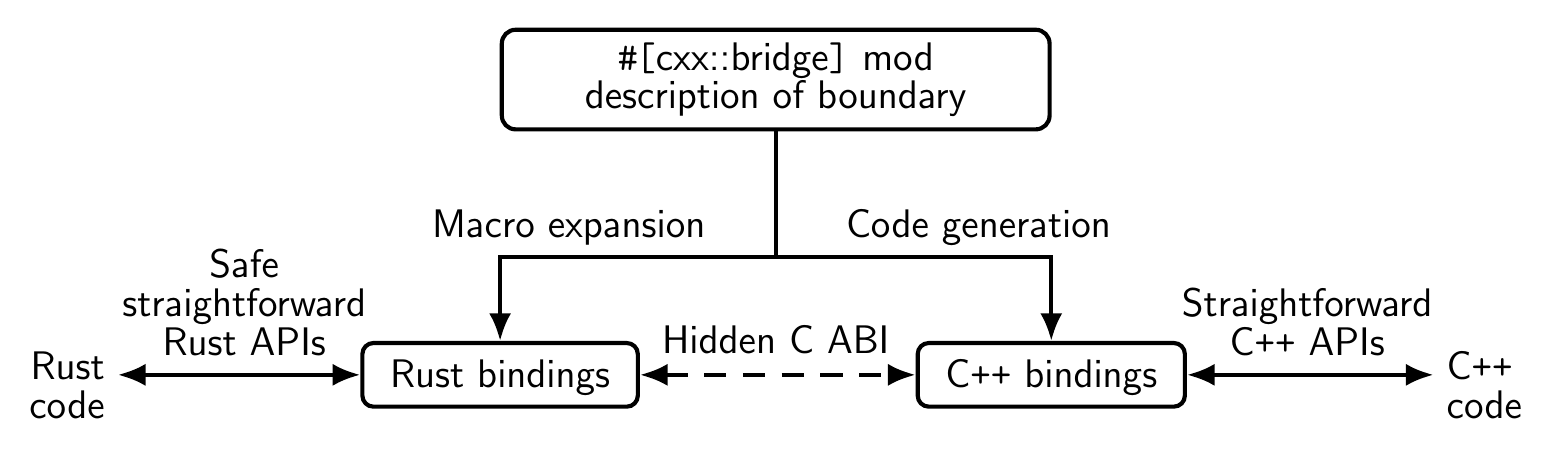
\begin{tikzpicture}[
  x=1cm,
  y=-.6cm,
  every node/.append style={
    line width=1.5pt,
    font=\Large\sansmath\sffamily,
  },
  every path/.append style={
    >={Latex[length=10pt,width=8pt]},
    line width=1.5pt,
  },
  execute at end node={\vphantom{bg}},
]
\node[draw, rounded corners=5, inner xsep=30pt, inner ysep=2pt]
  (bridge) at (0, .25) {\makecell{\texttt{\#\hspace{-1pt}[}cxx::bridge\texttt{]} mod\\[-4pt]description of boundary}};
\node[draw, rounded corners, inner xsep=10pt, inner ysep=6pt, text depth=1pt]
  (rust-bindings) at (-3.5, 6.5) {Rust bindings};
\node[draw, rounded corners, inner xsep=10pt, inner ysep=6pt, text depth=1pt]
  (cpp-bindings) at (3.5, 6.5) {C\texttt{++} bindings};
\node[inner xsep=4pt, inner ysep=-0pt]
  (rust-code) at (-9, 6.5) {\makecell[r]{\\[-8pt]Rust\\[-4pt]code}};
\node[inner xsep=4pt, inner ysep=-0pt]
  (cpp-code) at (9, 6.5) {\makecell[l]{\\[-8pt]C\texttt{++}\\[-4pt]code}};
\draw (bridge) -- (0, 4);
\draw[<->] (rust-bindings) |- (0, 4) -| (cpp-bindings);
\draw[<->] (rust-code) -- (rust-bindings);
\draw[<->, dash pattern=on 8pt off 6pt] (rust-bindings) -- (cpp-bindings);
\draw[<->] (cpp-bindings) -- (cpp-code);
\draw (-.75, 4) node[anchor=south east] {Macro expansion};
\draw (.75, 4) node[anchor=south west] {Code generation};
\draw (0, 6.5) node[anchor=south, inner ysep=4pt] {Hidden C ABI};
\draw (-6.75, 6.5) node[anchor=south, inner ysep=1pt] {\makecell{Safe\\[-4pt]straightforward\\[-4pt]Rust APIs}};
\draw (6.75, 6.5) node[anchor=south, inner ysep=1pt] {\makecell{Straightforward\\[-4pt]C\texttt{++} APIs}};
\pgfresetboundingbox\path
  (-9.5, 0) -- (rust-bindings.south)+(0, .3) -- (9.5, 0) -- (bridge.north);
\end{tikzpicture}
\end{document}
